Lämpöpumppujen käyttö kiinteistöjen lämmitykseen kasvattaa suosiotaan(Lähde, lukumäärät). Lämpöpumppu saattaa olla kiinteistön ainut lämmitysmuoto, tai se saattaa toimia toisten lämmitysjärjestelmien rinnalla. Lämpöpumpuilla voidaan korvata vanha järjestelmä, millä on vaikutusta kiinteistön lämmityksen aiheuttamaan sähkönkulutuksen luonteeseen.

\section{Lämpöpumpun toimintaperiaate}
  Lämpöpumpun eli jäähdytyskoneen toimintaperiaate on käänteinen lämpövoimakoneelle. Lämpöpumppu siirtää lämpöenergiaa viileämmästä ympäristöstä lämpimämpään.

  Lämpöpumpun perusrakenne koostuu kompressorista, lauhduttimesta, paisuntaventtiilistä ja höyrystimestä, joiden välillä kiertää kylmäaine. Järjestelmä on kuvattu kuvassa \ref{fig:hptp}. Matalassa paineessa oleva kylmäaine höyrystyy viileämmässä tilassa sijaitsevassa höyrystimessä ja vastaannottaa lämpöenergiaa. Höyrystynyt kylmäaine johdetaan lauhduttimeen ja sen paine nostetaan kompressorin avulla korkeammaksi, jolloin sen lämpötila nousee. Korkeassa paineessa ja lämpötilassa oleva kylmäaine luovuttaa lämpöenergiaa lauhduttimen välityksellä lämpimään ympäristöön, jolloin osa siitä nesteytyy. Nesteytynyt kylmäaine virtaa paisuntaventtiilin kautta takaisin höyrystimeen. Paisuntaventtiilissä kylmäaineen paine ja täten myös lämpötila laskevat.

  Höyrystimessä lämpöenergiaa siirtyy kylmäaineeseen ympäristöstä. Lämmön kuljettaminen ympäristöstä lauhduttimelle voidaan toteuttaa erilaisilla tavoilla. Suomessa yleisin tapa on käyttää ilmapuhallinta \parencite{lähde}, joka puhaltaa ulkoilmaa höyrystimen lävitse ja jäähdyttää sitä. Tällöin kyseessä on ilmalämpöpumppu. Toinen yleinen vaihtoehto on käyttää maahan kaivettavaa tai kallioon porattaaa lämmönkeruuputkistoa. Tälläistä lämpöpumppua kutsutaan maalämpöpumpuksi. Eri sovelluskohteissa käytetään myös lukuisia muitakin lämmönlähteitä kuten ilmanvaihdon poistoilmaa, viemärivettä, lauhdevettä tai vesistöä\parencite{lähde}.

  Lauhduttimessa kylmäaineen luovuttama lämpöenergia siirretään sovelluskohteesta riippuen esimerkiksi käyttöveteen, lämmitysjärjestelmän vesikiertoon tai suoraan huoneilmaan. Teollisuudessa tuotettua energiaa voidaan käyttää esimerkiksi erilaisissa prosesseissa. Sovelluskohde määrää lauhduttimelta vaadittavan lämpötilan. Järjetelmiä saatetaan kutsua erilaisilla nimillä riippuen siitä, mihin tuotetteua energiaa käytetään. Mikäli tuotettulla energialla lämmitetään käyttövettä tai lämmitysjärjetelmän kiertovettä, kutsutaan laitetta Ilma--vesilämpöpumpuksi\parencite{lähde}.

  \begin{figure}
    \centering
    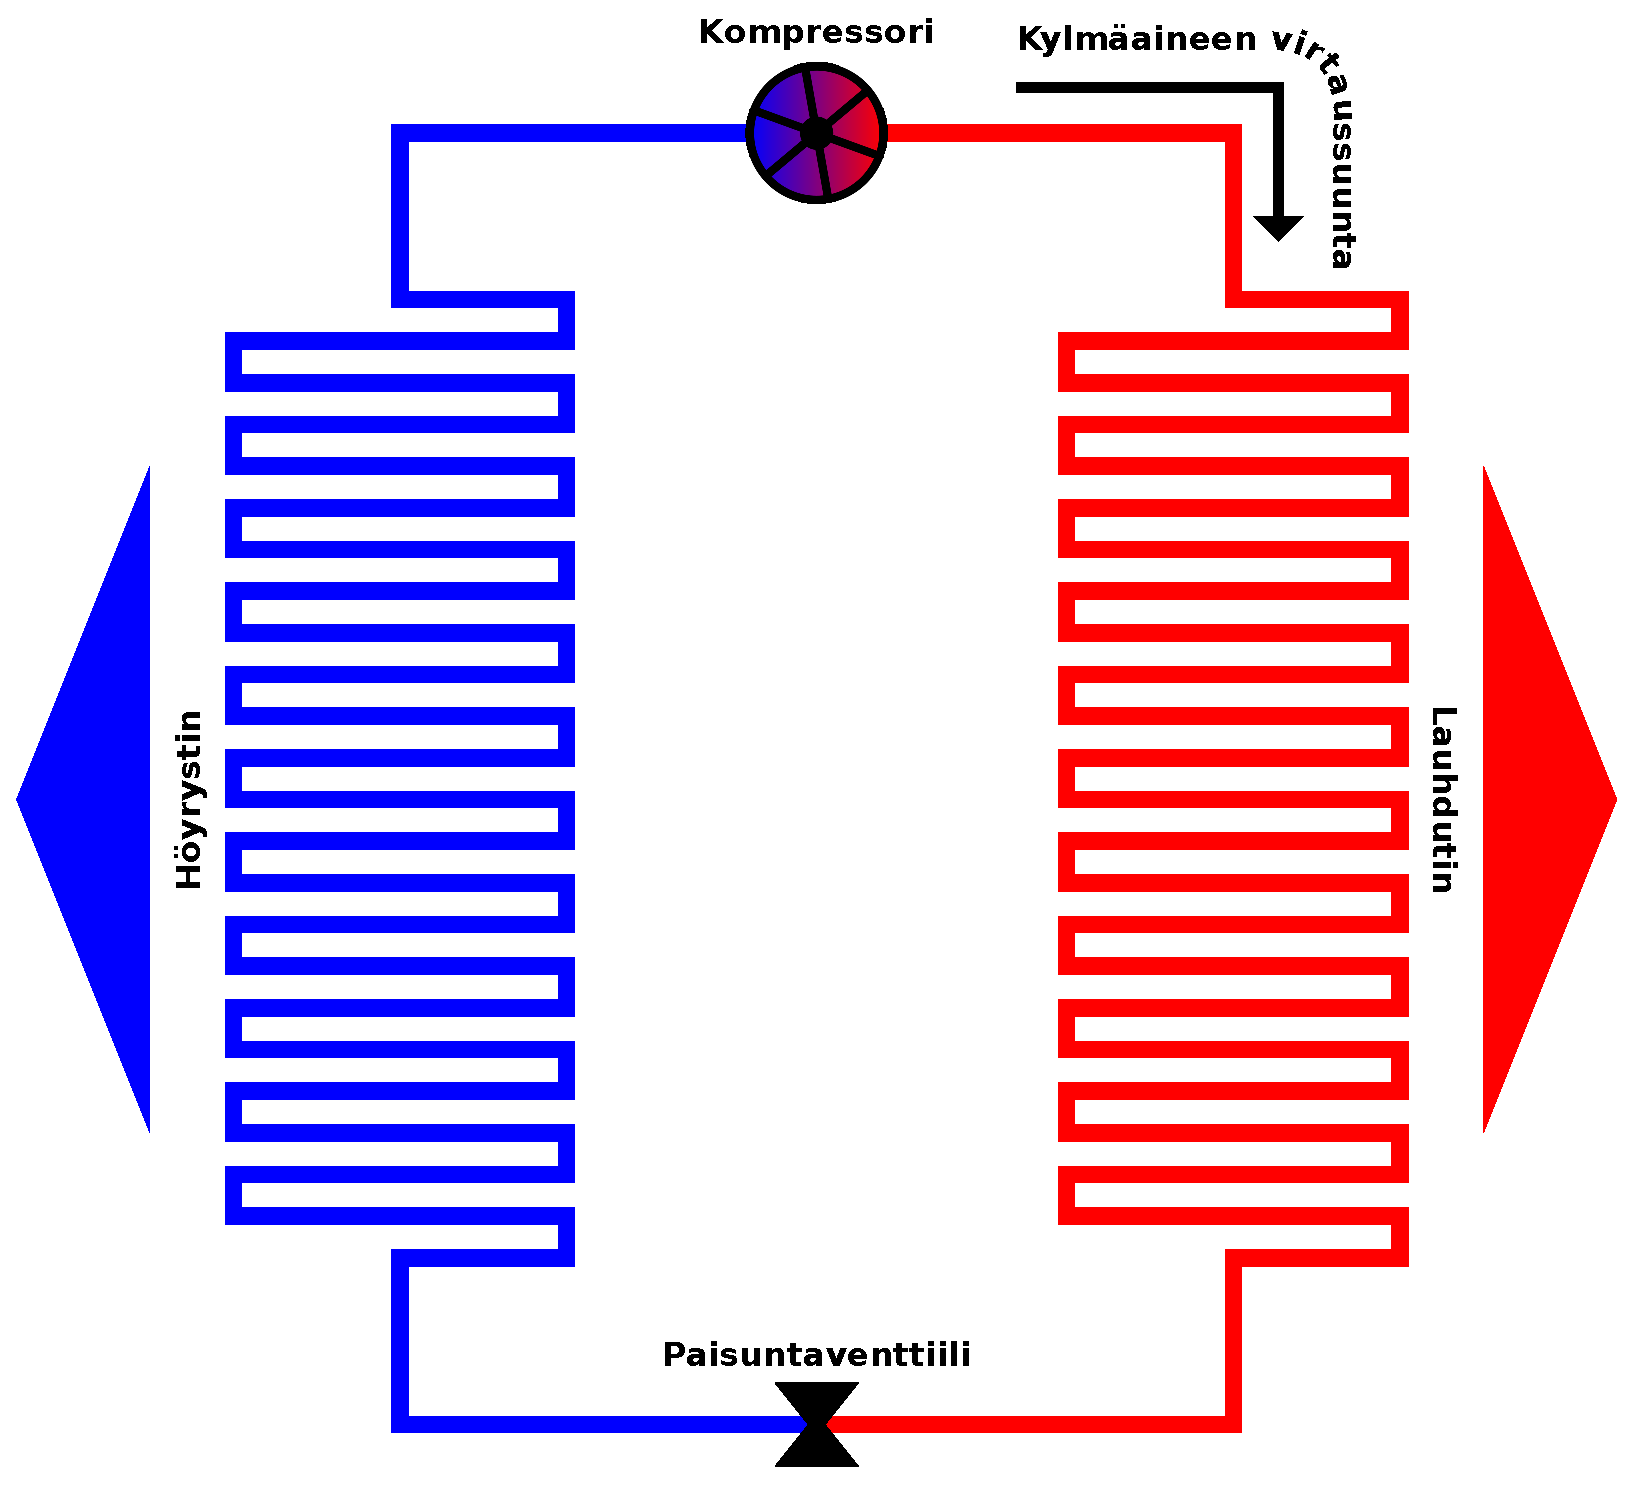
\includegraphics[width=0.5\textwidth]{figures/hp}
    \caption{Lämpöpumpun toimintaperiaate}
    \label{fig:hptp}
  \end{figure}

  Lämpöpumput käyttävät sähköenergiaa lämmön siirtämiseen viileämmästä lämpövarastosta lämpimämpään. Käytetystä sähköenergiasta valtaosa kuluu paineen tuottamiseen kompressorilla, mikä ylläpitää energiaa tuottavaa työkiertoa. Kompressorin lisäksi sähköä kuluu pienempiä määriä vaikkapa lämpöpumpun ohjaukseen, lämmitysjärjestelmän kiertovesipumpun käyttämiseen tai ilmalämpöpumpun sisäyksikön puhaltimen käyttämiseen. Mikäli lämpöpumpun teho on mitoitettu pienemmäksi kuin suurin vaadittu lämmitysteho\footnote{osatehomitoitus}, voidaan tehojen erotus tuottaa tarvittaessa lämpöpumpun yhteyteen asennettavilla sähkövastuksilla. Tälläinen ratkaisu lisää huomattavasti järjestelmän sähkönkulutusta suurimman energiantarpeen aikana, käytännössä kovilla pakkasilla.



  
